%%%%%%%%%%%%%%%%%%%%%%%%%%%%%%%%%%%%%%%%%
% baposter Landscape Poster
% LaTeX Template
% Version 1.0 (11/06/13)
%
% baposter Class Created by:
% Brian Amberg (baposter@brian-amberg.de)
%
% This template has been downloaded from:
% http://www.LaTeXTemplates.com
%
% License:
% CC BY-NC-SA 3.0 (http://creativecommons.org/licenses/by-nc-sa/3.0/)
%
%%%%%%%%%%%%%%%%%%%%%%%%%%%%%%%%%%%%%%%%%

%----------------------------------------------------------------------------------------
%	PACKAGES AND OTHER DOCUMENT CONFIGURATIONS
%----------------------------------------------------------------------------------------

\documentclass[a0paper,fontscale=0.29]{baposter} 


\usepackage{amsmath,amsfonts,amssymb}
\usepackage{amsthm}
\usepackage[utf8]{inputenc}
\usepackage{xspace}
\usepackage{dsfont}
\usepackage{color}
\usepackage[overlay,absolute]{textpos}
\usepackage{stmaryrd}
\usepackage{ifthen}
\usepackage{mathtools}
\usepackage{enumitem}
\usepackage{url}
\usepackage{hyperref}
\usepackage{cleveref}
\hypersetup{
	colorlinks,
	citecolor=black,
	filecolor=black,
	linkcolor=black,
	urlcolor=black
}

\usepackage{tikz}
\usetikzlibrary{shapes,calc,snakes,decorations,arrows}

\usepackage{graphicx} % Required for including images
\usepackage{booktabs} % Top and bottom rules for tables
\usepackage{enumitem} % Used to reduce itemize/enumerate spacing
\usepackage{palatino} % Use the Palatino font
\usepackage[font=small,labelfont=bf]{caption} % Required for specifying captions to tables and figures
\definecolor{lightblue}{rgb}{0.145,0.6666,1} % Defines the color used for content box headers

\usepackage{multicol} % Required for multiple columns
\setlength{\columnsep}{1.5em} % Slightly increase the space between columns
\setlength{\columnseprule}{0mm} % No horizontal rule between columns

\newcommand{\compresslist}{ % Define a command to reduce spacing within itemize/enumerate environments, this is used right after \begin{itemize} or \begin{enumerate}
			\setlength{\itemsep}{1pt}
			\setlength{\parskip}{0pt}
			\setlength{\parsep}{0pt}
		}
		%-----unnumerated-----
		\newtheorem*{definition*}{Definition}
		\newtheorem*{notation*}{Notation}
		\newtheorem*{lemma*}{Lemma}
		\newtheorem*{remark*}{Remark}
		\newtheorem*{corollary*}{Corollary}
		\newtheorem*{theorem*}{Theorem}
		\newtheorem*{proposition*}{Proposition}
		\newtheorem*{claim*}{Claim}
		\newtheorem*{example*}{Example}
		\newtheorem*{exercise*}{Exercise}

\usepackage{caladea}
\usepackage[T1]{fontenc}

\usepackage{setspace}
\usepackage{xcolor}
\usepackage{qrcode}
\usepackage{multicol}
\usepackage{enumitem,xcolor}
\usepackage{booktabs}
\usepackage{tabularx}

\definecolor{lightgray}{gray}{0.8}
\definecolor{lightcyan}{rgb}{0.84,1,1}
\definecolor{lightgreen}{rgb}{0.64,1,0.71}
\definecolor{lightred}{rgb}{1,0.7,0.71}
\definecolor{tured}{HTML}{C40D20}
\definecolor{tuorange}{HTML}{ff6e00}
\definecolor{tuored}{HTML}{E23E10}
\definecolor{tugrey}{HTML}{444444}
\definecolor{tugrey2}{HTML}{b2b2b2}
\definecolor{tuviolet}{HTML}{8f13fc}
\definecolor{tublue}{HTML}{1f91cc}
\definecolor{tugreen}{HTML}{47cb3f}

\setlist[itemize]{leftmargin=*}
\renewcommand{\labelitemi}{$\triangleright$}
\renewcommand{\labelitemii}{$\triangleright$}
\renewcommand{\labelitemiii}{$\triangleright$}
\renewcommand{\labelitemiv}{$\triangleright$}


\begin{document}
\def\mystrut(#1,#2){\vrule height #1pt depth #2pt width 0pt}   

\begin{poster}
{
grid=false,
columns=6,
headerborder=closed, % Adds a border around the header of content boxes
colspacing=1.1em, % Column spacing
rowspacing=2.2em,
bgColorOne=white, % Background color for the gradient on the left side of the poster
bgColorTwo=white, % Background color for the gradient on the right side of the poster
borderColor=tured, % Border color
headerColorOne=tured, % Background color for the header in the content boxes (left side)
headerColorTwo=tured, % Background color for the header in the content boxes (right side)
headerFontColor=white, % Text color for the header text in the content boxes
boxColorOne=white, % Background color of the content boxes
textborder=roundedsmall, % Format of the border around content boxes, can be: none, bars, coils, triangles, rectangle, rounded, roundedsmall, roundedright or faded
eyecatcher=true, % Set to false for ignoring the left logo in the title and move the title left
headerheight=16em, % Height of the header
headershape=rectangle, % Specify the rounded corner in the content box headers, can be: rectangle, small-rounded, roundedright, roundedleft or rounded
headerfont=\Large, % Large, bold and sans serif font in the headers of content boxes
%textfont={\setlength{\parindent}{1.5em}}, % Uncomment for paragraph indentation
linewidth=2pt % Width of the border lines around content boxes
}
%----------------------------------------------------------------------------------------
%	TITLE SECTION 
%----------------------------------------------------------------------------------------
%
{
\hspace*{1.5cm}    
\includegraphics[height=6.5em]{images/sect.png}
} % First university/lab logo on the left
{
{\Huge{\strut{\normalfont \mystrut(1,1) \textbf{What All the PHUZZ Is About:}  \\ \mystrut(1,10) \huge A Coverage-guided Fuzzer for Finding \\ Vulnerabilities in PHP Web Applications \mystrut(1,5)}  }}
\vspace{0.5em}
} % Poster title
{
\normalfont{{\underline{Sebastian Neef}, Lorenz Kleissner, Jean-Pierre Seifert}} \\ SecT, Technische Universität Berlin, Germany \\
{\small @ CSAW'24 - Grenoble INP/ESISAR, Valence, France - 08.11.2024}
}{

\includegraphics[height=5.5em]{images/tublogo.png} \hspace*{2cm}
} % Second university/lab logo on the right

\headerbox{{Challenges}}{name=challenges,column=2,row=0,span=2,headerColorOne=tugrey,headerColorTwo=tugrey,borderColor=tugrey}{
\begin{enumerate}[leftmargin=*]\compresslist
    \item \textbf{How to find endpoints and parameters?}
    \begin{itemize}\compresslist
        \item Comprehensive fuzzing of the application?
    \end{itemize}
    \item \textbf{How to mutate the input?}
    \begin{itemize}\compresslist
        \item Adherence to HTTP protocol?
        \item Correct parameter to endpoint mapping?
    \end{itemize}
    \item \textbf{How to collect coverage \& feedback?}
    \begin{itemize}\compresslist
        \item Instrumentation of high-level PHP code?
        \item Coverage without shared memory?
    \end{itemize}
    \item \textbf{How to detect web vulnerabilities?}
    \begin{itemize}\compresslist
        \item Alternatives to missing \emph{''crash''} indicator?
    \end{itemize}
\end{enumerate}
}

\headerbox{{Motivation}}{name=motivation,column=0,row=0,span=2,headerColorOne=tugrey,headerColorTwo=tugrey,borderColor=tugrey,bottomaligned=challenges}{
\begin{center}
    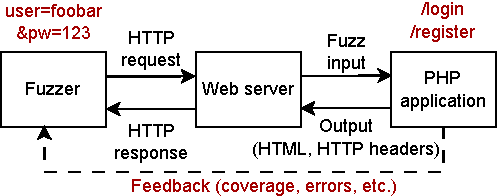
\includegraphics[width=\textwidth]{images/webfuzzer-minified.drawio-crop.pdf}
\end{center}

\begin{itemize}
    \item Fuzzing $\triangleq$ Automated software testing
    \item Extensively researched for binary software
    \item Little research on fuzzing web applications
\end{itemize}
}


\headerbox{{Contributions}}{name = solutions, column = 4, row = 0,span=2,bottomaligned=challenges,headerColorOne=tugrey,headerColorTwo=tugrey,borderColor=tugrey}{
\vspace{0.2cm}
\begin{itemize}
    \item \textbf{PHUZZ} framework for fuzzing PHP web apps
    \item Browser-based approach for more control over fuzzed endpoints and parameters
    \item Simplified instrumentation without code changes to fuzz target or PHP interpreter
    \item Vulnerability detection that supports \\ SQLi$^\star$, RCE$^\star$, XXE$^\star$, insecure deserialization$^\star$, path traversal$^\star$, open redirection$^\dagger$, XSS$^\dagger$
    \item Support for parallel fuzzing
\end{itemize}
}


\headerbox{{Implementation \& Components of PHUZZ}}{name = phuzz, column = 0, span = 4, row = 1, below=motivation,headerColorOne=tured,headerColorTwo=tured,borderColor=tured}{ %bottomaligned = challenges
\begin{center}
    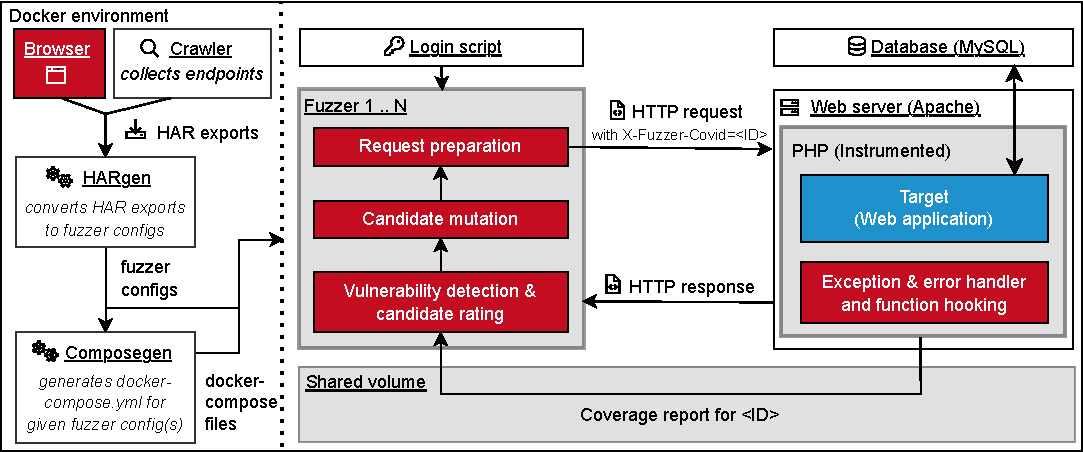
\includegraphics[width=\linewidth]{images/fuzzerdetail-minified-v3.drawio-crop.pdf}
\end{center}
\vspace{-0.7cm}
\begin{itemize} \compresslist
    \item Dockerized \& modular design for enhanced usability and extensibility
\end{itemize}
}


\headerbox{{Instrumentation}}{name = fhooking, column = 4, row = 1, span=2, below=solutions, bottomaligned=phuzz,headerColorOne=tured,headerColorTwo=tured,borderColor=tured}{
\begin{center}
    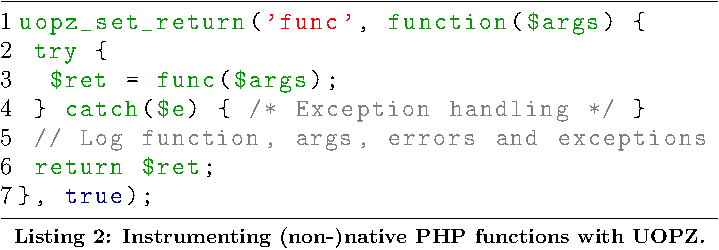
\includegraphics[width=\textwidth]{images/phuzz-listing2-crop.pdf}
\end{center}
\vspace{-0.6cm}
\begin{itemize}
    \item Transparent function hooking of (non-)native PHP functions using UOPZ extension
    \item Transparent coverage collection using pcov or \\ Xdebug extensions
    \item Observe dangerous functions, triggered errors and exceptions  
    \item Increase coverage by overriding and disabling authentication and authorization functions
\end{itemize}
}


\headerbox{{PHUZZ Discovers Zero-day Vulnerabilities}}{name = 0vulns, column = 3, span = 3, row = 2, below=phuzz,headerColorOne=tured
,headerColorTwo=tured,borderColor=tured}{
    \begin{center}
        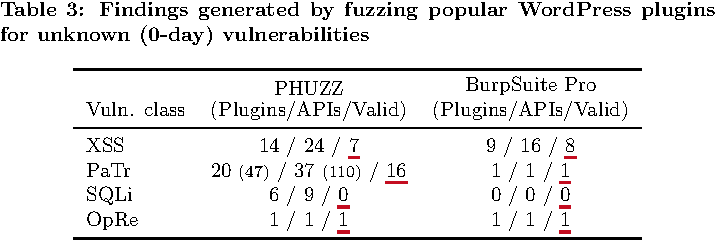
\includegraphics[width=\linewidth]{images/table3-crop.pdf}
    \end{center}
    \vspace*{-0.5cm}
    \begin{itemize}
        \item \textbf{Proof of concepts for two exploitable vulnerabilities}:
        \vspace*{-0.20cm}
        \begin{itemize} \compresslist
            \item[$\rightarrow$] CVE-2023-6294: popup-builder SSRF \& Arbitrary File Read
            \item[$\rightarrow$] CVE-2023-6295: so-widgets-bundle Local File Inclusion
        \end{itemize}
    \end{itemize}
}


\headerbox{{PHUZZ Outperforms Other Vulnerability Scanners}}{name = kvulns, column = 0, span = 3, row = 2, below=phuzz,headerColorOne=tured,headerColorTwo=tured,borderColor=tured,bottomaligned=0vulns}{
    \begin{center}
        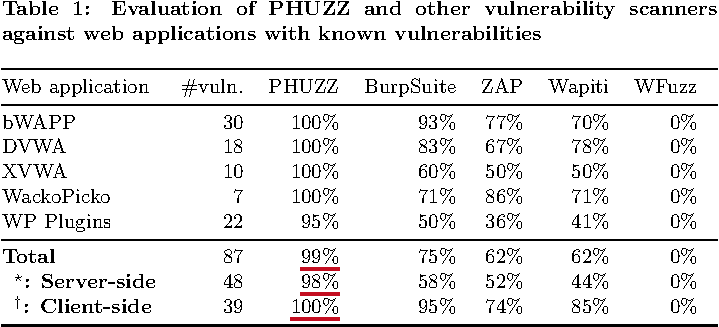
\includegraphics[width=\linewidth]{images/phuzz-table1-crop.pdf}
    \end{center}
}

\headerbox{{More Information}}{name = info, column = 4, span=2, row = 3, below = 0vulns,headerColorOne=tuorange,headerColorTwo=tuorange,borderColor=tuorange}{ %aligned=exact, above=bottom}{
\begin{multicols}{2}
    \begin{center}
            \qrcode[padding]{https://doi.org/10.1145/3634737.3661137} \\ Link to full paper \vfill 
            \columnbreak
            \qrcode[padding]{https://github.com/gehaxelt/phuzz} \\ Link to repository \vfill
    \end{center}
\end{multicols}
\begin{center}
Contact: neef@tu-berlin.de
\end{center}
}

\headerbox{{ Conclusions}}{name = conclusion, column = 0, row = 3, span=4, below = kvulns, bottomaligned = info,headerColorOne=tuorange,headerColorTwo=tuorange,borderColor=tuorange}{
\begin{itemize}
    \item Coverage-guided fuzzing presents a powerful method for uncovering web vulnerabilities.
    \item The \textsc{PHUZZ} framework effectively identifies seven distinct vulnerability classes, all without altering the web application's code, PHP interpreter, or external components.
    \item \textsc{PHUZZ} has proven its real-world effectiveness by uncovering previously unknown vulnerabilities.
    \item To support ongoing research, we have made all related code and data publicly available.
    \item We encourage future research to build upon and expand \textsc{PHUZZ}, advancing this field further.
\end{itemize}
}

\end{poster}
\end{document}
